\section{Results}





% \begin{table}
% \centering
% \caption{Execution time as a function of $n$. Each datapoint consists of 10,000 samples.}
% \begin{tabular}{|l|c|c|c|c|} \hline
% Method\textbackslash Range&(2-500)&(501-5000)&(5001-50000)&(50001-500000) \\
% \hline
% AKS&6.55E9&-&-&-\\ \hline
% MR&1.86E-2&1.94E-2&2.11E-2&2.19E-2\\ \hline
% SS&2.20E-2&2.52E-2&2.82E-2&3.15E-2\\ \hline
% TD&3.61E-3&4.65E-3&6.36E-3&1.03E-2\\ \hline
% WS&1.06E-2&1.26E-2&1.44E-2&1.74E-2\\ \hline
% \end{tabular}
% \label{tab:pressure}
% \end{table}


\begin{table}
\centering
\caption{Execution time as a function of $n$. Each datapoint consists of 10,000 samples.}
\begin{tabular}{|l|c|c|c|c|c|} \hline
Range\textbackslash Method&AKS&MR&SS&TD&WS \\ \hline
2-500&6.55E9&1.86E-2&2.20E-2&3.61E-3&1.06E-2 \\ \hline
501-5000&-&1.94E-2&2.52E-2&4.65E-3&1.26E-2 \\ \hline
5001-50000&-&2.11E-2&2.82E-2&6.36E-3&1.44E-2 \\ \hline
50001-500000&-&2.19E-2&3.15E-2&1.03E-2&1.74E-2 \\ \hline
\end{tabular}
\label{tab:pressure}
\end{table}


% \begin{table}
% \centering
% \caption{Error as a function of $n$. Each datapoint consists of 10,000 samples. All methods have a one-sided error: they may say ``prime'', while it is a composite.}
% \begin{tabular}{|l|c|c|c|c|} \hline
% Method\textbackslash Range&(2-500)&(501-5000)&(5001-50000)&(50001-500000) \\
% \hline
% AKS&0&-&-&-\\ \hline
% MR&1.27E-2&2.64E-3&1.11E-3&1.09E-4\\ \hline
% SS&9.52E-3&2.99E-3&5.53E-4&0\\ \hline
% TD&0&0&0&0\\ \hline
% WS&0&0&0&0\\ \hline
% \end{tabular}
% \label{tab:pressure}
% \end{table}




\begin{table}
\centering
\caption{Error (fraction) as a function of $n$. Each datapoint consists of 10,000 samples. All methods have a one-sided error: they may say ``prime'', while it is a composite.}
\begin{tabular}{|l|c|c|c|c|c|} \hline
Range\textbackslash Method&AKS&MR&SS&TD&WS \\ \hline
2-500&0&1.27E-2&9.52E-3&0&0 \\ \hline
501-5000&-&2.64E-3&2.99E-3&0&0 \\ \hline
5001-50000&-&1.11E-3&5.53E-4&0&0 \\ \hline
50001-500000&-&1.09E-4&0&0&0 \\ \hline
\end{tabular}
\label{tab:pressure}
\end{table}



\begin{figure}
	\centering
	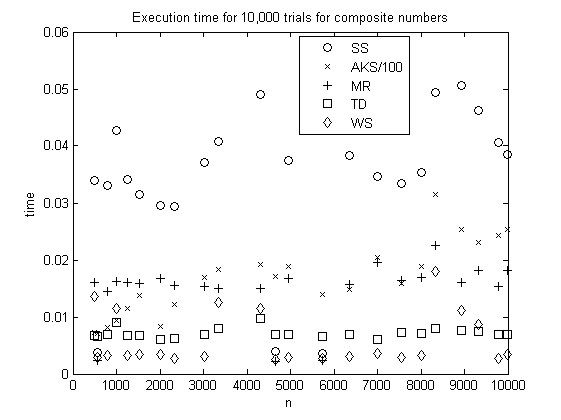
\includegraphics[width=0.5\textwidth]{../Graphs/ExecutionTime1.png}
	\caption{Execution time for small composite numbers, $n$. Each measurement consists of 10,000 samples.}
	\label{fig:executionTime1}
\end{figure}


\begin{figure}
	\centering
	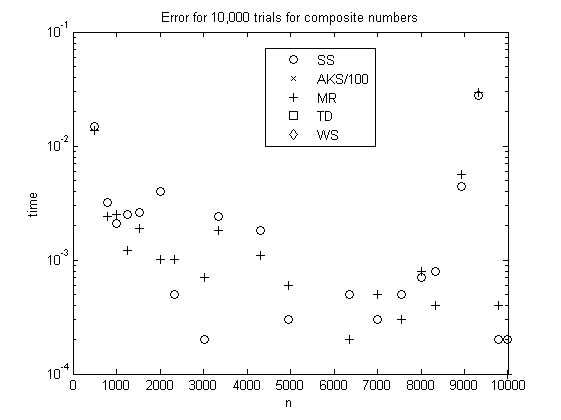
\includegraphics[width=0.5\textwidth]{../Graphs/Error1.png}
	\caption{Error (false prime prediction) for small composite numbers, $n$. Each measurement consists of 10,000 samples.}
	\label{fig:error1}
\end{figure}


\begin{figure}
	\centering
	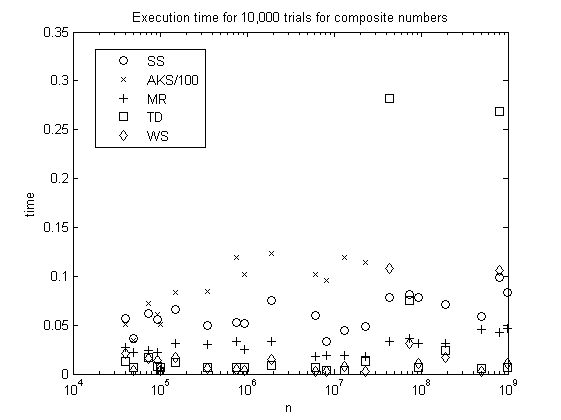
\includegraphics[width=0.5\textwidth]{../Graphs/ExecutionTime2.png}
	\caption{Execution time for a large range of composite numbers, $n$. Each measurement consists of 10,000 samples.}
	\label{fig:executionTime2}
\end{figure}



\begin{figure}
	\centering
	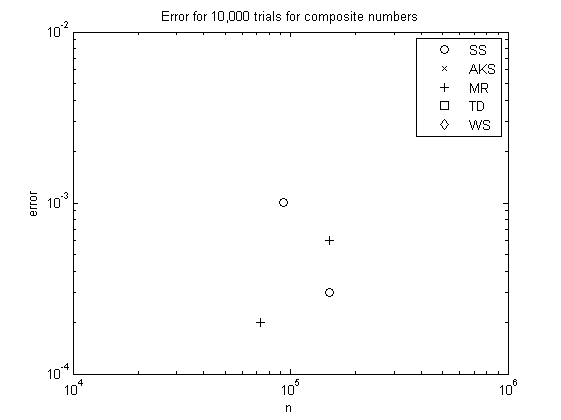
\includegraphics[width=0.5\textwidth]{../Graphs/Error2.png}
	\caption{Error (false prime prediction) for a large range of composite numbers, $n$. Each measurement consists of 10,000 samples.}
	\label{fig:error2}
\end{figure}

